\subsection{Metric} 
%Semantic similarity of source code can be estimated via the similarity in term of different levels: lexical, syntax, and structural. Based on those three levels, we provide three metrics 
%

Remind that our goal of the experiment is to (in)validate whether BLEU reflects the semantic accuracy of the migrated code from the tools with respect to the manual-migrated code in the collected ground truth. In our experiment, however, we will also study to verify the uses of three other metrics to estimate the semantic accuracy. Those metrics are associated with three levels of representations of source code: String Edit Distance (SED) that associates with lexical level, Tree Edit Distance (TREED) that associates with syntax, and Graph Vector Edit Distance (GVED) that associates with structural analysis. We will provide their correlation result with semantic accuracy in Section 5 and those metrics are the backbone of our proposed solution in Section 6. In this section, we will define and give examples for those metrics. 

\subsubsection{\textbf{String Edit Distance (SED)}} This metric measures effort that a user must edit in term of the code tokens
that need to be deleted/added in order to transform the
resulting code into the correct one. It is computed as:  $SED = \frac{EditDistance\left(s_R, s_T\right)}{length\left(s_R\right)}$ where $EditDistance\left(s_R, s_T\right)$ is the editing distance between each pair of the reference method $s_R$ and the translated method $s_T$; and the denominator is the total length of the referenced method. The metrics is also normalized in 0-1 range. 

\subsubsection{\textbf{Tree Edit Distance (TREED)}}  
The sematical quality of translated code depends on its syntax. Until now, abstract syntax trees(AST) are structures widely used in  representing the syntax of programming code. Therefore, computing the difference of two ASTs is considered as the evaluating method of syntax difference.
In this study, we apply this in measuring the difference between the syntax of referenced method and translated method. Given a pair of method in C\# which are need to be compared their syntax, Roslyn[cite here] is used to parse them into ASTs. Then we compute the tree edit distance between two trees using the algorithm Treed described in the paper \cite{algorithm}.
To be more detailed, the tree edit distance is calculated by number of operations (add/delete/replace/move) to make them identical. 

It is computed as:  $TREED = 1 -  \frac{TreeEditDistance\left(AST_R, AST_T\right)}{CountNodes \left(AST_R+AST_T\right)}$ where $TreeEditDistance\left(AST_R, AST_T\right)$ is the editing distance between two trees of referenced method $AST_R$ and the translated method $AST_T$; and the denominator is the total nodes in the tree of both two methods. The value of TREED is from 0 to 1. For any two trees, there will always exist at least one editing (such as the one that deletes all nodes of the first tree and inserts all the nodes of the second). Therefore, there will always exist at least one TREED value and the higher value is, the more similar those trees are.

\begin{figure}[h]
	\caption{Tree Editing Example: In the label of each node, its type is in capital font and its val (if exists) is in normal font}
	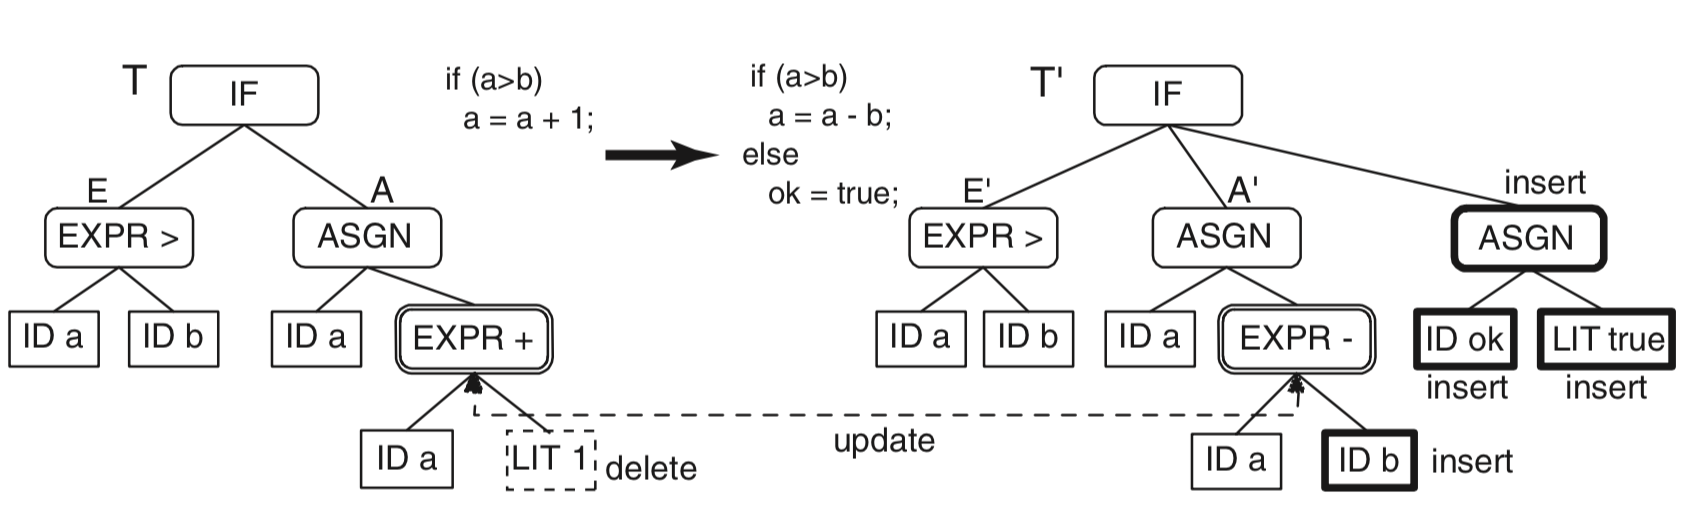
\includegraphics[scale=0.3]{img/treed.png}
	\centering
	\label{fig:treed}
\end{figure}

In the example in Figure 1, an \textit{if} statement was edited by modifying the \textit{if} branch and adding an \textit{else} branch. The two trees represent the two versions of a method. An editing consists of one \textit{Delete} (dotted line box), one \textit{Update} (double-line box), and four \textit{Insert} operations (bold boxes). Other nodes (single- line boxes) are either unchanged or moved. Based on the formula TREED, the result of TREED in this case  $TREED = 1 - \frac{1 + 1 + 4}{16}=0.625$





\subsubsection{\textbf{Graph Vector Edit Distance (GVED)}} 

Structure-oriented approaches in code semantic comparision have become
popular. Among those approaches, Exas is an accurate and efficient
structural characteristic feature extraction approach that better
approximates and captures the structure within the fragments of
artifacts~\cite{fase09}.  In our study, we use Exas as a mean of
computing the difference between code structures. Given a pair of
method in C\# which are need to be compared their structure, program
dependence graphs (PDGs) are built with some additional nodes from
GROUM~\cite{fse09}. Exas vectors will be computed on those graphs. In
Exas, the characteristic features are extracted from the patterns of
elements of the graphs. The code fragments are characterized by their
counting vectors of those features. The difference between two vectors
reflects the difference of two graphs.

%Therefore, distance of these counting vectors is considered the way to measure the sematic between code fragments.

Figure~\ref{fig:PDGs} shows the PDGs of the code fragments 1 and
2. These graphs are analysed by Exas, which focuses on two kinds of
patterns of structural information of the graph, called $(p,q)$-node
and $n$-path as can be seen in Table~\ref{tab:feature1} and
Table~\ref{tab:feature2}.

An efficient way to express the property ``having the same or similar
features'' is to use vectors. The characteristic vector of a
fragment is the occurrence-count vector of its features. That is, each
position in the vector is indexed for a feature and the value at that
position is the number of occurrences of that feature in the
fragment. Table~\ref{tab:featureIndex} shows the indexes of the
features, which are global across all vectors. Based on the occurrence
counts, the vectors for code fragment 1 and 2 are
$V_1$(1,1,1,1,1,0,1,0...),$V_2$(1,1,0,1,1,1,1,1...), respectively. Two
fragments having the same feature sets and occurrence counts will have
the same vectors and vice versa. The vector similarity can be measured
by a chosen vector distance such as 1-norm distance.

We introduce the formula for normalizing the result of vector edit
distance which is used in our experiments. The normalized
value is described as
\[GVED \left( V_1, V_2 \right) = 1 - \sum_{i=1}^{n} \frac{ \mid XV1_i - XV2_i \mid}{XV1_i + XV2_i}\], 
where $n$ denotes the number of vector scalar, $V_1$ denotes the
counting vector of the first graph, $V_2$ denotes the counting vector
of the second graph, $XV1_i$ denotes $V_1$\rq the value of the ($i-th$)
scalar, $XV2_i$ denotes $V2$\rq the value of the ($i-th$) scalar.

In this example in Figure~\ref{code1code2}, the value of GVED is $GVED\left(V_1, V_2\right) = 1 - \frac{8 }{20} = 0.6 $,

\begin{figure}
\begin{lstlisting}[language=JAVA]
	Code 1:
	void foo(int i) {
		int j;
		if (i < 2) {
			j = 1;
		} else {
			j = 2;
		}
	}

	Code 2:
	void foo(int i) {
		int j;
		if (i < 2) 
			j = i;	 
		j = 2;
	}
\end{lstlisting}
\caption{Example of two code fragments}
\label{code1code2}
\end{figure}

\begin{figure}[h]
	\caption{An example: two PDGs represent code1 and code2}
	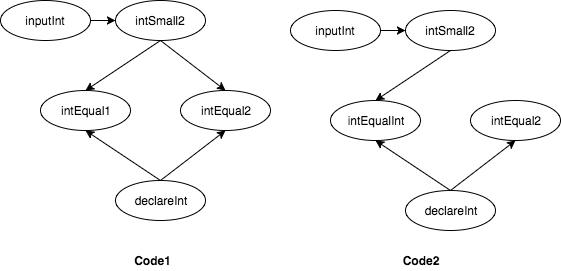
\includegraphics[scale=0.4]{img/Diagram_PDG.png}
	\centering
	\label{fig:PDGs}
\end{figure}

% Table generated by Excel2LaTeX from sheet 'Sheet1'
\begin{table}[htbp]
  \centering
  \caption{Feature table of code1 extracted in Exas}
  \scalebox{0.65}{
    \begin{tabular}{|l|l|l|l|l|r|}
    \toprule
    \textbf{Pattern} & \multicolumn{5}{c|}{\textbf{Feature of Code1}} \\
    \midrule
    \textit{\textbf{1-path}} & inputInt & intSmall2 & intEqual1 & intEqual2 & \multicolumn{1}{l|}{declareInt} \\
    \midrule
    \textit{\textbf{2-path}} & \multicolumn{1}{p{6.415em}|}{inputInt-intSmall2} & \multicolumn{1}{p{5.915em}|}{intSmall2-intEqual1} & \multicolumn{1}{p{6em}|}{intSmall2-intEqual2} & \multicolumn{1}{p{5.75em}|}{declareInt-intEqual1} & \multicolumn{1}{p{5em}|}{declareInt-intEqual2} \\
    \midrule
    \textit{\textbf{3-path}} & \multicolumn{1}{p{6.415em}|}{intputInt-intSmall2-intEqual1} & \multicolumn{1}{p{5.915em}|}{intputInt-intSmall2-intEqual2} &       &       &  \\
    \midrule
    \textit{\textbf{(p,q)-node}} & inputInt-0-1 & intSmall2-1-2 & intEqual1-2-0 & intEqual2-1-2 &  \\
    \bottomrule
    \end{tabular}%
	}
  \label{tab:feature1}%
\end{table}%

% Table generated by Excel2LaTeX from sheet 'Sheet1'
\begin{table}[htbp]
  \centering
	\caption{Feature table of code2 extracted in Exas}
	\scalebox{0.65}{
	    \begin{tabular}{|l|l|l|l|l|r|}
    \toprule
    \textbf{Pattern} & \multicolumn{5}{c|}{\textbf{Feature of Code2}} \\
    \midrule
    \textit{\textbf{1-path}} & inputInt & intSmall2 & intEqualInt & intEqual2 & \multicolumn{1}{l|}{declareInt} \\
    \midrule
    \textit{\textbf{2-path}} & \multicolumn{1}{p{6.415em}|}{inputInt-intSmall2} & \multicolumn{1}{p{5.915em}|}{intSmall2-intEqualInt} & \multicolumn{1}{p{6em}|}{declareInt-intEqual1} & \multicolumn{1}{p{5.75em}|}{declareInt-intEqual2} &  \\
    \midrule
    \textit{\textbf{3-path}} & \multicolumn{1}{p{6.415em}|}{intputInt-intSmall2-intEqualInt} &       &       &       &  \\
    \midrule
    \textit{\textbf{(p,q)-node}} & inputInt-0-1 & intSmall2-1-1 & intEqualInt-2-0 & intEqual2-1-0 &  \\
    \bottomrule
    \end{tabular}%
	}
  \label{tab:feature2}%
\end{table}%

% Table generated by Excel2LaTeX from sheet 'Sheet1'
\begin{table}[htbp]
	\centering
	\caption{Feature Indexing}
	\scalebox{0.75}{
	\begin{tabular}{|cccc|}
		\toprule
		\multicolumn{1}{|l|}{\textbf{Feature}} & \multicolumn{1}{l|}{\textbf{Index}} & \multicolumn{1}{l|}{\textbf{Counted in Code1}} & \multicolumn{1}{l|}{\textbf{Counted in Code2}} \\
		\midrule
		\multicolumn{1}{|l|}{inputInt} & \multicolumn{1}{r|}{1} & \multicolumn{1}{r|}{1} & \multicolumn{1}{r|}{1} \\
		\midrule
		\multicolumn{1}{|l|}{intSmall2} & \multicolumn{1}{r|}{2} & \multicolumn{1}{r|}{1} & \multicolumn{1}{r|}{1} \\
		\midrule
		\multicolumn{1}{|l|}{intEqual1} & \multicolumn{1}{r|}{3} & \multicolumn{1}{r|}{1} & \multicolumn{1}{r|}{0} \\
		\midrule
		\multicolumn{1}{|l|}{intEqual2} & \multicolumn{1}{r|}{4} & \multicolumn{1}{r|}{1} & \multicolumn{1}{r|}{1} \\
		\midrule
		\multicolumn{1}{|l|}{declareInt} & \multicolumn{1}{r|}{5} & \multicolumn{1}{r|}{1} & \multicolumn{1}{r|}{1} \\
		\midrule
		\multicolumn{1}{|l|}{intEqualInt} & \multicolumn{1}{r|}{6} & \multicolumn{1}{r|}{0} & \multicolumn{1}{r|}{1} \\
		\midrule
		\multicolumn{1}{|p{5.75em}|}{inputInt-intSmall2} & \multicolumn{1}{r|}{7} & \multicolumn{1}{r|}{1} & \multicolumn{1}{r|}{1} \\
		\midrule
		\multicolumn{1}{|l|}{intEqual2-1-0} & \multicolumn{1}{r|}{8} & \multicolumn{1}{r|}{0} & \multicolumn{1}{r|}{1} \\
		\midrule
		\multicolumn{4}{|c|}{To be continued} \\
		\bottomrule
	\end{tabular}%
	}
	\label{tab:featureIndex}%
\end{table}%


\subsubsection{\textbf{Semantic Score}}
\begin{table}
\caption{Manual Semantic Score Criteria}
\begin{tabular}{|c|p{6.5cm}|}
\hline
Score & Description \\
\hline
0 & The translated method is totally useless. One needs to rewrite the whole method. \\
\hline
1 & The translated method seems to be incorrect. Even though some parts are reusable, it is not worth to fix and use the method. \\
\hline
2 &  It cannot be decided if the translated method is useful or not. \\
\hline
3 & The translated method seems to be correct. Even though it needs some adjustments, it is worth to use the method. \\
\hline
4 & The methods are identical in term of functionality. There is no change needed and it can be use as-is. \\
\hline
\end{tabular}
\label{table:criteria}
\end{table}

%\textbf{Semantic Score.}
%To answer the question whether BLEU score reflect semantic of source code,
%Before one can answer the question whether BLEU score reflects semantic accuracy of translated source code or not, it is necessary to define what is the semantic accuracy. Given a pair of methods: one generated by SMT-based migration system and another one is the reference code written by real developers, the semantic accuracy is expressed by the similarity in term of functionality between the two. If the two methods perform the same functionality, they are semantically similar.

%
Semantic accuracy between pairs of methods (one is the result from a
SMT-based migration tool and another is the reference code from the
ground truth) is the similarity between them in term of execution and
functionality. If two methods perform similar operations on a given
input, they are semantically similar, even interchangeable. A pair of
methods can have the same functionality despite of their difference in
term of program elements.
%
For example, a method using a \code{for} loop and a method using a
\code{while} loop, they still can perform the same functionality even
though their lexical representations are much different. There exist
many studies aiming to measure the functionality similarity of source
code, which utilize the similarities of structures and
dependencies~\cite{clone-tse07,roy09,ducasse99,baker97,ccfinder,cpminer,baxter98,deckard,deckard2,horwitz01}.
%
However, they are not reliable as their results sometimes contradict
with human judgments on semantic accuracy~\cite{fse14-higo}. More
importantly, those structure-based metrics {\em do not reflect human
  efforts} in fixing the incorrect migrated code into the correct one.
%
Human judgment for our study would be the most reliable metric to
measure semantic accuracy. A developer who examines a pair of methods
can tell whether the code perform the same functionality as well as
explain the efforts needed for the correction. Therefore, we conducted
a study that used a human subject to manually evaluate the migrated
code from the SMT-based migration tools.
%2 goals

%Our study was conducted as follows:

\emph{1. Sample Size}. Because our dataset contains a large number of
pairs of code, it would take a lot of efforts to manually evaluate all
of them. According to \cite{website}, from a population of 34,209, a
sample size of 375 is acceptable with the confidence level of 95\% and
the margin of error of 5\%. Therefore, we randomly sampled 375 pairs
of methods from the dataset for evaluation.

\emph{2. Setting}. The human subject of our study is one of the
authors who is fluent in both Java and C\#. He was then given a pair
of methods in C\#: one was the translated method generated by an SMT
tool and another one was the reference code originally written by
developers.
% (for example: a pair of method in figure xxx). Each method
%was labeled clearly as reference or machine-generated code.
He was also given the original Java code to understand the
requirements of the migration task for this method. Moreover, he was
provided with the github links to the corresponding projects where
those methods came from (with both Java and C\# versions) so that he
would have a better context of the migrated code.

\emph{3. Scoring.} Finally, the human subject was told to give a score
for each of 375 pairs of methods. We set two goals for the human
subject in evaluating the results. The first goal is the correctness of
the resulting code with respect to the manual-migrated code in the
ground truth. The second one is based on the efforts needed to correct
the translated code to achieve the same functionality as of the
reference code in the ground truth.
%
%The scoring was based on the human efforts needed to fix the
%translated method to achieve the same functionality as of the
%reference one.

Score ranges from 0 to 4 as follows:

\begin{compactitem}

\item A score of 0 means the translated code is totally useless, and
  it is better to re-write the whole method rather than use it.

\item A score of 1 means the translated method seems to be incorrect, and even
though some parts of it are reusable, the human subject do not want to
fix and use it.

\item A score of 2 means the human subject cannot decide whether to
  use the translated method or not.

\item A score of 3 means the translated method seems to be correct,
  but it still needs some minor adjustments.

\item A score of 4 means the pairs of methods are identical in term of
functionality, and the translated method can be used as-is.

\end{compactitem}

In short, the scoring guidelines are listed on
Table~\ref{table:criteria}. Before actually giving the scores, the
human subject could study our preselected examples with according
scores and explanation. The examples are presented on
Figure~\ref{fig:scoreEG}. Specifically, the code from line 11 to line
20 represents a result with a score of 4. Noted that even though it is
different from the reference code in term of actual program elements
(use a regular \code{for} loop, instead of a \code{foreach}), it still
performs the same functionality. A translated method of score 3 (lines
21 to line 30) seems to have similar functionality as the reference
code, but it still needs minor editing (line 23 contains an incorrect
function call, \code{indexOf} instead of \code{IndexOf} with an
incorrect parameter). Lines 31 to 40 demonstrates a translated method
which has score of 3. It cannot be decided if the method should be
used or not. It has some good program elements that are similar to the
reference code, but at the same time, has some critical errors that
would be hard to fix. A translated method of score 1 (lines 41 to 50)
has only one line of code that is reusable (line 43). So it is not
worth fixing/reusing the code. Lines 51 to 60 represents a translated
code of score 0 which means the entire translated code is totally
useless, \ie it is better to rewrite the whole method.

%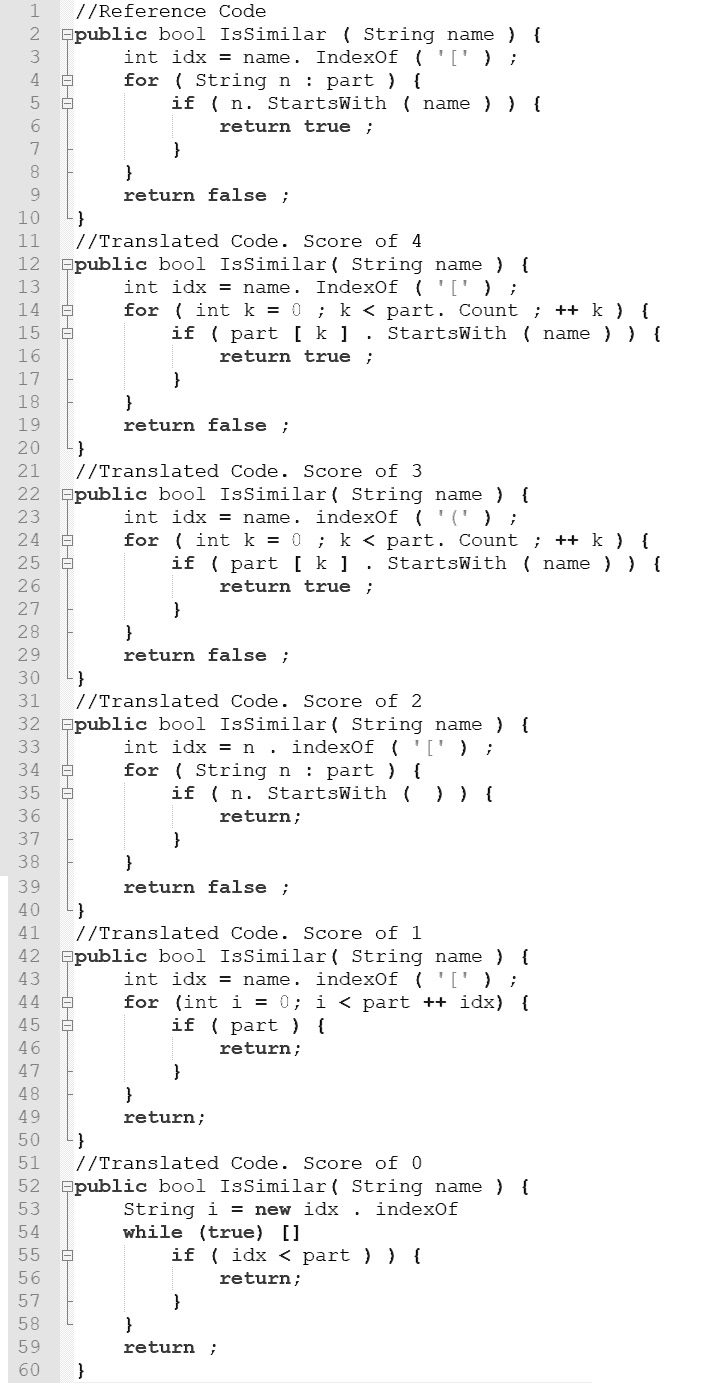
\includegraphics{scoreExamples}

We conducted the same human study for the results of both lpSMT and mppSMT models. As a result, we have scores for 375 pairs of methods for each model. From now on, we regard those scores as \textbf{semantic score}.

\begin{figure}
\caption{Scoring Examples}
\centering
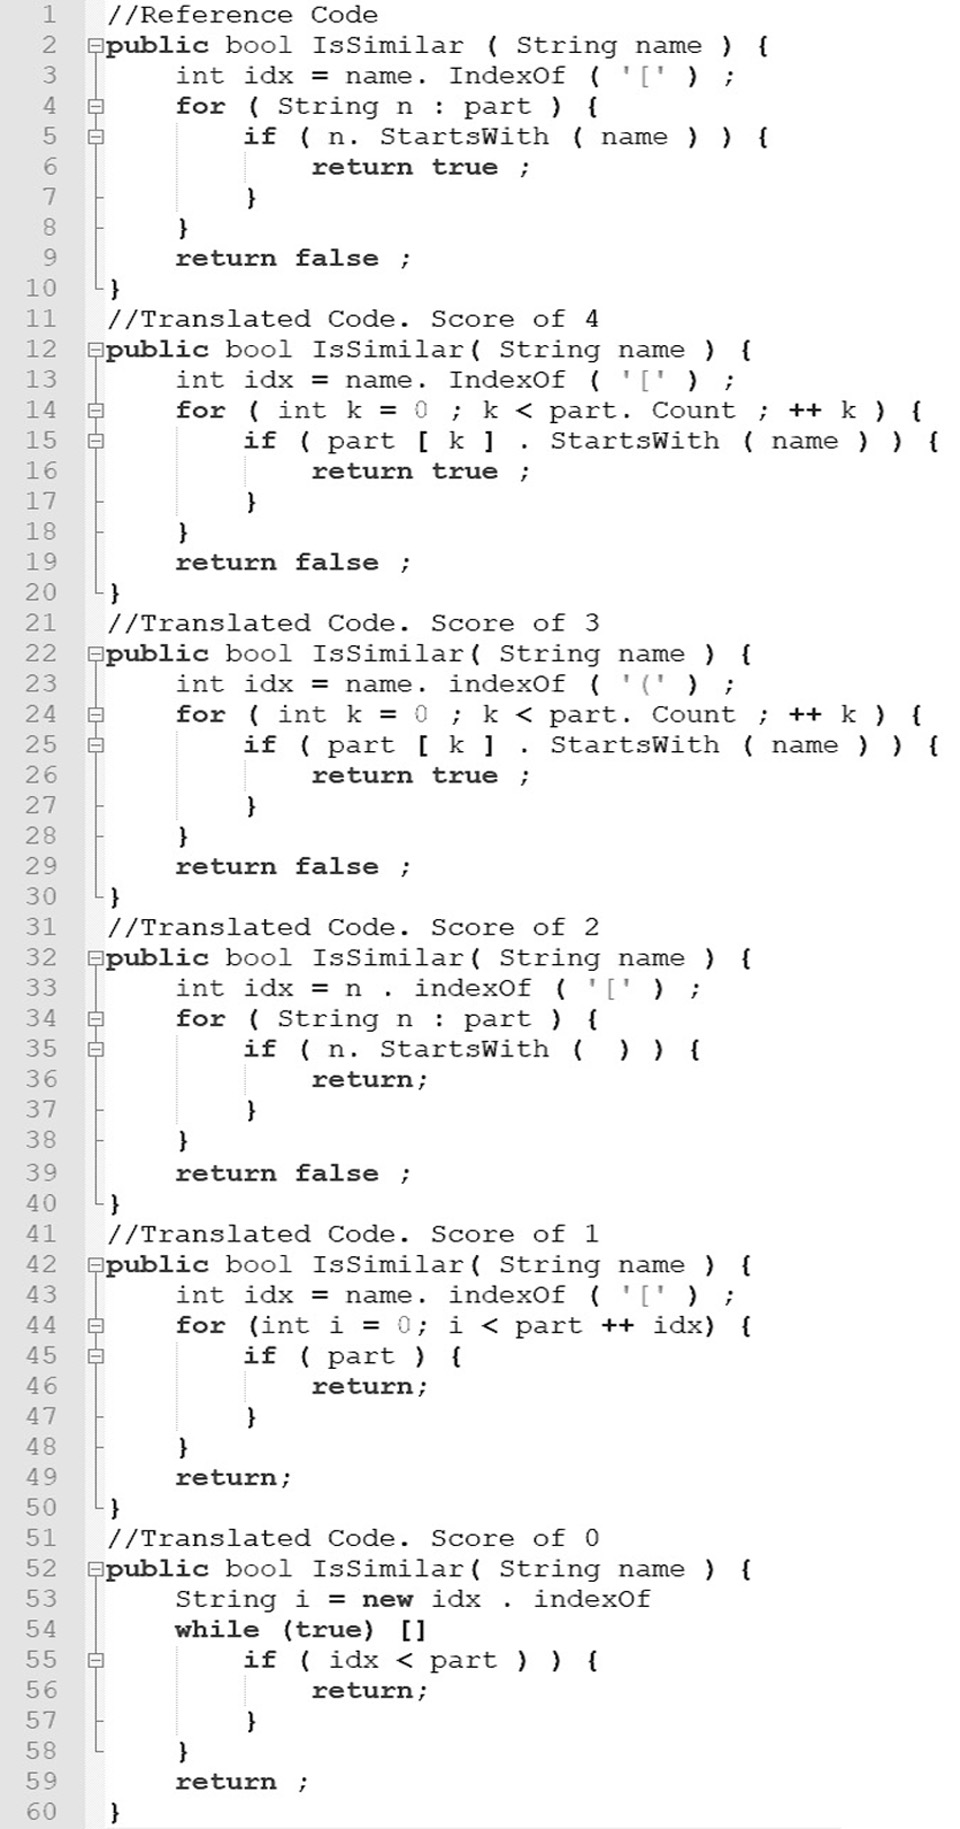
\includegraphics{img/scoreExamples}
\label{fig:scoreEG}
\end{figure}


%Our hypothesis states that \emph{\textit{BLEU score does not measure well the similarity in term of semantics between the reference and migrated source code}}. Therefore, given a pair of methods (reference one and machine translated one), we need a metric that can measure the similarity in term of semantics between them. As we know of, there is no automated metrics to do that task. To determine semantic similarity score, we used a human subject to manually evaluate pairs of methods to see how close they are in term of semantic/functionality. Specifically, scoring is done based on the human effort to fix the translated method to achieve the same functionality as of the reference one. The detailed scoring guidelines are presented in Table\ref{table:criteria}. The human subject is a senior developer who is fluent in both Java and C\#. He was given a pair of methods in C\# (machine generated one and reference one), the original method in Java, and the context project from which the methods come from. Then, he was told to evaluate pairs of methods in C\#, and give score as our guideline above and table \ref{table:criteria}. He could also refer back to the original Java method and project for a better understanding of the context. Below are examples for each score from -2 to 2:\\
%To determine semantic similarity score between pair of methods, we manually scored each pair from 0 to 6 based on the human effort to fix a translated method to a referenced one. Specifically, we list the criteria to score in Table  with a score of 0 means the pair of methods are totally different, and a score of 6 means they are totally the same. Scoring also follows the following principles: 1. An effort to fix a syntactical error (misplacing a semi-colon, parenthesis...) has less weight than an effort to fix a semantical error (wrong branch, wrong function call...). 2. A fix that requires adding sources code has more weight than one that requires removing/replacing. 3. A fix for user-defined program elements (identifier, simple name, method name) is more 'pricey' than a fix for keyword (this, if, for...). Example (of scores 1,3,5).

%Since our dataset contains a large number of pairs of methods, it would take a lot of efforts to manually evaluate all of them. Hence, we took a sample from our population of total 34,209 pairs. According to \cite{website}, our sample size is 375 with confidence level of $95\%$ and margin of error $5\%$. After we conducted the human experiment with 375 pairs of methods, we normalized the result on 0-1 range with 0 is respected to -2 and 1 is respected to 2.
